\section{Detailed proofs of lemmas and theorems}
\textbf{Proof of Theorem~\ref{thm:alphacpnoise}}
Fix any $\mc S \subseteq \mc X$. Let $\mc C^*_S = \{S_1^*, \ldots, S_k^*\}$ be a clustering of $\mc S$ such that $m(\mc C_{\mc S}^*) = t$ and $\mc C^*_S$ has $(\alpha, \eta)$-center proximity. Denote by $r_i := r(S_i^*)$ and $r = \max r_i$. Define $Y_B^{\mc C} := \{C_i \in \mc C : C_i \subseteq B \text{ or } |B \cap C_i| \ge t/2\}$. Note that whenever a ball $B$ satisfies the sparse-distance condition, all the clusters in $Y_{B}^{{\mc C}^{(l)}}$ are merged together and the clustering $\mc C^{(l+1)}$ is updated. We will prove the theorem by proving two key facts.

\begin{enumerate}[nolistsep, noitemsep, label=\textbf{F.\arabic*},leftmargin=0.3in]
\renewcommand\labelitemi{$\diamond$}
\item \label{fact:1} If the algorithm merges points from a good cluster $S_i^*$ with points from some other good cluster,  then at this step the distance being considered $d = d(p,q) > r_i$.	
\item \label{fact:2} When the algorithm considers the distance $d = r_i$, it merges all points from $S_i^*$ (and possibly points from $\mc X\setminus \mc S$) into a single cluster $C_i$. Hence, there exists a node in the tree $N_i$ which contains all the points from $S_i^*$ and no points from any other good cluster $S_j^*$. 	
\end{enumerate}
Note that the theorem follows from these two facts. Similar reasoning was also used in proof of Lemma 3 in \cite{balcan2012clustering}. We now prove both of these facts formally. 

\noindent\textit{\underline{Proof of Fact.~\ref{fact:1}}}
Let $\mc C^{(l)} = \{C_1, \ldots, C_{k'}\}$ be the current clustering of $\mc X$. Let $l+1$ be the first merge step which merges points from the good cluster $S_i^*$ with points from some other good cluster. Let $p, q \in \mc X$ be the pair of points being considered at this step and $B = B(p, d(p, q))$ the ball that satisfies the sparse distance condition at this merge step. Denote by $Y = Y_{B}^{C^{(l)}}$. We need to show that $d(p, q) > r_i$. To prove this, we need Claim~\ref{claim:fromBothCluster} below. 

\begin{smallLemma}
\label{claim:fromBothCluster}
Let $p, q \in \mc X$ and $B$, $Y$, $S_i^*$ and $C^{(l)}$ be as defined above. If $d(p, q) \le r,$ then $B \cap S_i^* \neq \emptyset$ and there exists $n \neq i$ such that $B \cap S_n^* \neq \emptyset$.
\end{smallLemma}
\vspace{-0.1in} $l+1$ is the first step which merges points from $S_i^*$ with some other good cluster. Hence, $\exists C_i \in Y$ such that $C_i\cap S_i^*  \neq \emptyset$ and $\forall n \neq i$, $C_i \cap S_n^* = \emptyset$. Also, $\exists C_j \in Y$ such that $C_j \cap S_j^* \neq \emptyset$ for some $S_j^*$ and $C_j \cap S_i^* = \emptyset$.

$C_i \in Y$. Hence, $C_i \subseteq B$ or $|C_i \cap B| \ge t/2$. The former is trivial. In the latter, for the sake of contradiction, assume that $B$ contains no points from $S_i^*$. This implies that $B \cap C_i \subseteq B \cap \{\mc X \setminus \mc S\}$ and $|B\cap \{\mc X \setminus \mc S\}| \ge t/2$. This  is a contradiction. The case when $C_j \in Y$ is identical. \qed

\begin{smallLemma}
\label{claim:maxrirj}
Let the framework be as given in Claim~\ref{claim:fromBothCluster}. Then, $d(p, q) > r_i$.
\end{smallLemma}

\vspace{-0.1in} \noindent If $d(p, q) > r$, then the claim follows trivially. In the other case, from Claim~\ref{claim:fromBothCluster}, $B$ contains $p_i \in S_i^*$ and $p_j \in S_j^*$. Let $r_i = d(c_i, q_i)$ for some $q_i \in S_i^*$.

$d(c_i, q_i) < \frac{1}{\alpha} d(q_i, c_j) < \frac{1}{\alpha} [ \frac{1}{\alpha}d(p_i, p_j) + \frac{1}{\alpha}d(c_i, q_i) + d(p_i, p_j) + 2d(c_i, q_i)]$
This implies that $(\alpha^2 - 2\alpha - 1)d(q_i, c_i) < (\alpha + 1) d(p_i, p_j)$. For $\alpha \ge 2 + \sqrt 7$, this implies that $d(c_i, q_i) < d(p_i, p_j)/2$ which implies $d(c_i, q_i) < d(p, q)$. This result was also stated in \cite{balcan2012clustering}.\qed

\noindent\textit{\underline{Proof of Fact \ref{fact:2}
}}
Let $\mc C^{(l)} = \{C_1, \ldots, C_{k'}\}$ be the current clustering of $\mc X$. Let $l+1$ be the merge step when $p = s_i$ and $q = q_i$ such that $d(s_i, q_i) = r_i$. We will prove that the ball $B = B(s_i, q_i)$ satisfies the sparse-distance condition.

\begin{smallLemma}
%\vspace{-0.1in}
\label{claim:dciqi}
Let $s_i$, $q_i$, $r_i$, $B$ and $Y$ be as defined above. Then, $B$ satisfies the sparse distance condition and for all $C \in Y$, for all $j \neq i, C \cap S_j^* = \emptyset$.
\end{smallLemma}
\vspace{-0.1in} $|B| = |S_i^*| \ge t$. Observe that, for all $C \in \mc C^{(l)}$, $|C| = 1$ or $|C| \ge t$. 

\begin{itemize}[nolistsep,leftmargin=*]
\item Case 1. $|C| = 1$. If $C \cap B \neq \emptyset \implies C \subseteq B = S_i^*$.
\item Case 2. $|C|\ge t$. $C \cap B \neq \emptyset$. Let $h(C)$ denote the height of the cluster in the tree $T$. 
\begin{itemize}[leftmargin=*]
\renewcommand\labelitemii{$\circ$}
\item Case 2.1. $h(C) = 1$. In this case, there exists a ball $B'$ such that $B' = C$. We know that $r(B') \le r_i \le r$. Hence using Claim~\ref{claim:maxrirj}, we get that for all $j \neq i$, $B' \cap S_j^* = \emptyset$. Thus, $|B'\setminus S_i^*| \le t/2 \implies |B\cap C| = |C| - |C\setminus B| = |C| - |B'\setminus S_i^*| \ge t/2$. Hence, $C \in Y$.

\item Case 2.2. $h(C) > 1$. Then there exists some $C'$ such that $h(C') = 1$ and $C' \subset C$. Now, using set inclusion and the result from the first case, we get that $|B\cap C| \ge |B\cap C'| \ge t/2$. Hence, $C \in Y$. Using Claim~\ref{claim:maxrirj}, we get that for all $j \neq i$, $C \cap S_j^* = \emptyset$.\qed\\
\end{itemize} 
\end{itemize}


\noindent\textbf{Proof of Theorem~\ref{thm:noalgalphacp}}
Let $\mc X, B_1, B_2, B_1', B_2'$ be as shown in Fig. \ref{fig:noalgalphacp}. Let $t_1 = \frac{t}{2}+1$ and $t_2 = \frac{t}{2}-2$. For $\alpha \le 2+\sqrt{3}$, clusterings $\mc C_{\mc S} = \{B_1, B_2, B_3, \ldots, B_k\}$ and $\mc C_{\mc S'} = \{\ B_1', B_2', B_3, \ldots, B_k\}$ satisfy $(\alpha, 1)$-center proximity and $m(\mc C_{\mc S}) = m(\mc C_{\mc S}') = t$. Now, a simple proof by contradiction shows that there doesn't exist a tree $T$ and prunings $P$ and $P'$ such that $P$ respects $\mc C_{\mc S}$ and $P'$ respects $\mc C_{\mc S'}$. \qed\\

\begin{figure}[!t]
\begin{center}
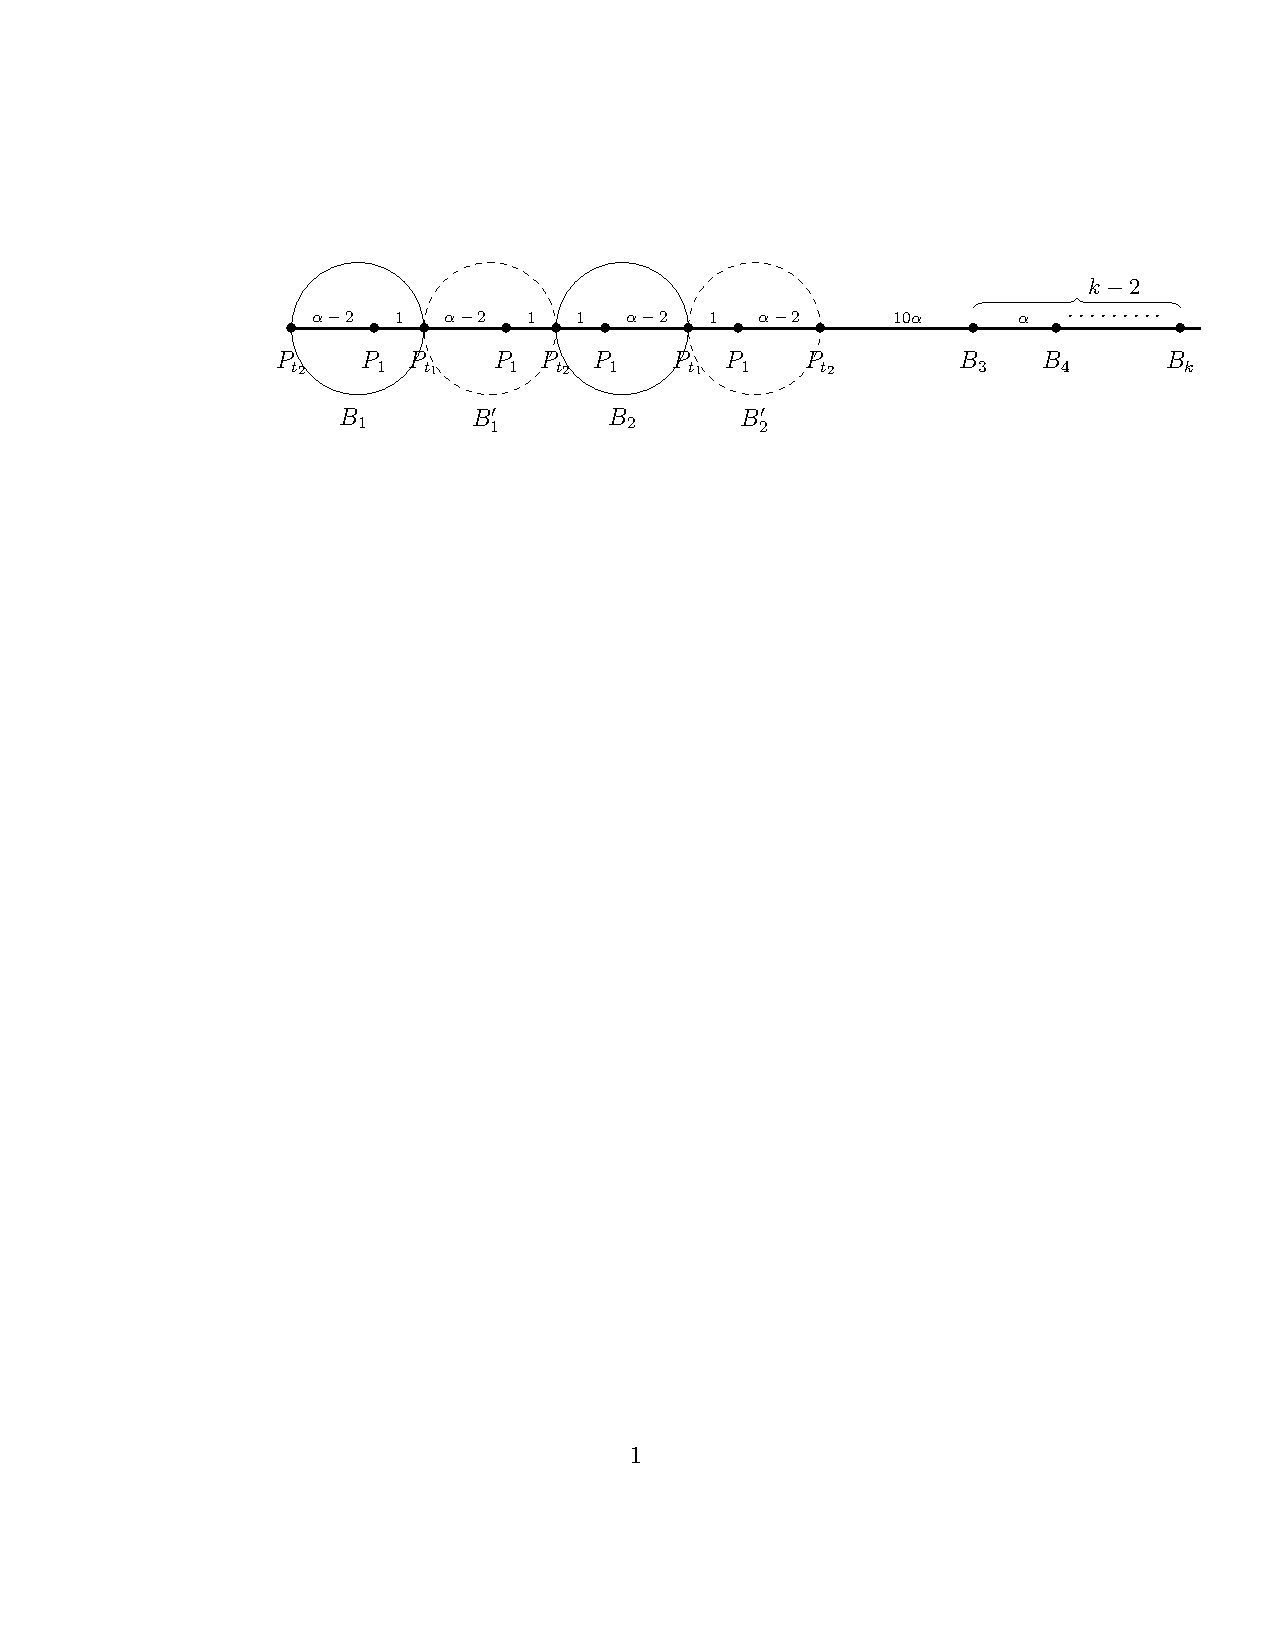
\includegraphics[trim={47mm 205mm 12mm 44mm},clip,width=\textwidth]{figures/clusteringNoise/lbdFig2.pdf}
\end{center}
\vspace{-1cm}
\caption{$\mc X \subseteq \mathbb{R}$ such that no tree can capture all the $(\alpha, \eta)$-proximal clusterings.}
\label{fig:noalgalphacp}
\end{figure}

\noindent\textbf{Proof of Theorem~\ref{thm:nolistalphacp}}
The clustering instance $\mc X$ is an extension of Fig. \ref{fig:noalgalphacp}. Let  $G_1 = \{B_1, B_1', B_2, B_2'\}$ be the balls as in Fig. \ref{fig:noalgalphacp}. Now, construct $G_2 = \{B_3, B_3', B_4, B_4'\}$ exactly identical to $G_1$ but far. In this way, we construct $k/2$ copies of $G_1$. \qed\\

\noindent\textbf{Proof of Theorem~\ref{thm:nosparsealg}}
Let $\mc X \subseteq \mathbb{R}$ be as shown in Fig. \ref{fig:nosparsealg}. Let $t' = \frac{t}{2}-1$ and let $B_1, B_2, B_3, B_1'$, $B_2', B_3', B_1'', B_2''$ and $B_3''$ be as shown in Fig.~\ref{fig:nosparsealg}. For $\alpha \le 2\sqrt{2}+3$, clusterings $\mc C_{\mc S} = \{B_1, B_2, B_3, \ldots, B_k\}$, $\mc C_{\mc S'} = \{\ B_1', B_2', B_3, \ldots, B_k\}$ and $\mc C_{\mc S}'' = \{\ B_1'', B_2'', B_3, \ldots, B_k\}$ satisfy $(\alpha, 1)$-center proximity. Also, $m(\mc C_{\mc S}) = m(\mc C_{\mc S}') =$ $m(\mc C_{\mc S}'') = t$. Arguing similarly as in Theorem \ref{thm:noalgalphacp} completes the proof. \qed\\
\begin{figure}[!t]
\vspace{-5mm}
\begin{center}
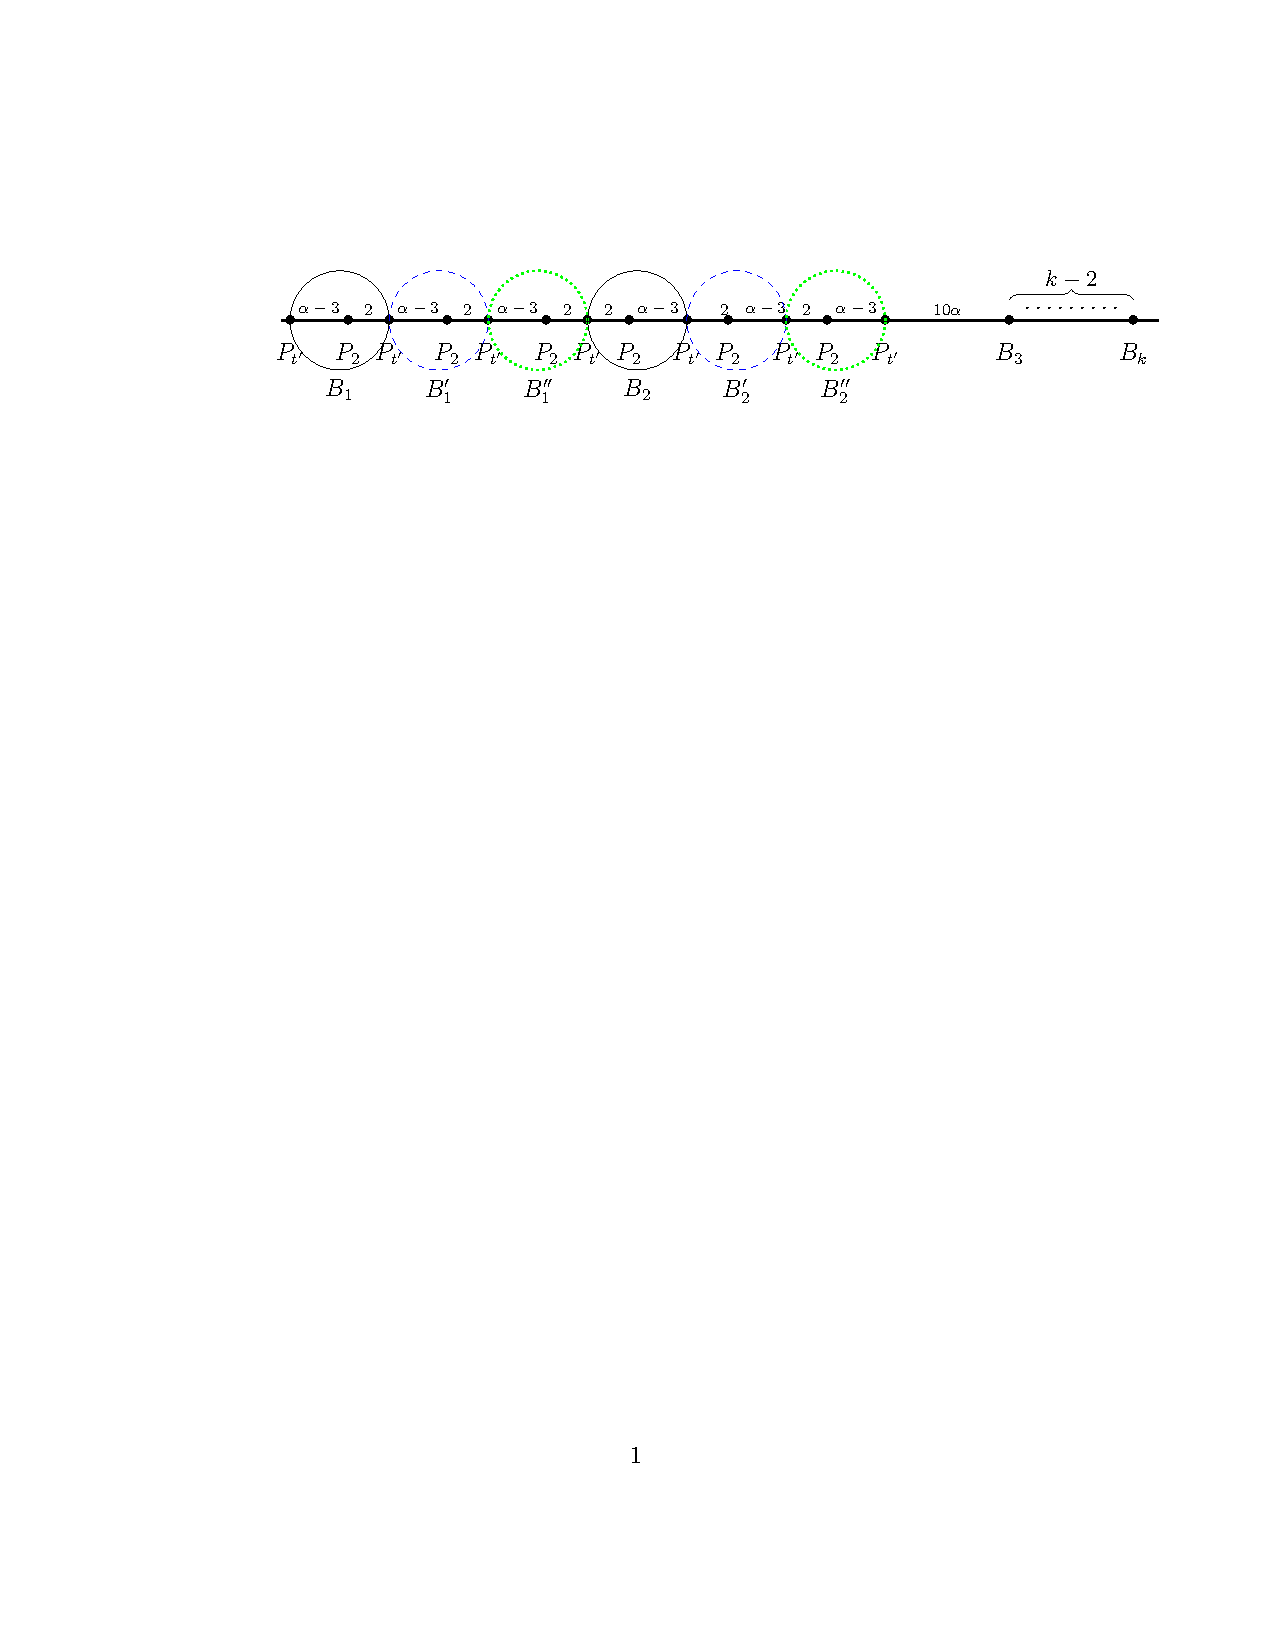
\includegraphics[trim={45mm 210mm 20mm 43mm},clip,width=\textwidth]{figures/clusteringNoise/lbdFig3.pdf}
\end{center}
\vspace{-4mm}
\caption{$\mc X \subseteq \mathbb{R}$ such that no algorithm can capture all the $\alpha$-proximal clusterings. } 
\label{fig:nosparsealg}
\end{figure}

\noindent\textbf{Proofs of Theorems~\ref{thm:nosparselistalphacp}, \ref{thm:nosparselistlambdacs} and \ref{thm:nolistlambdacs}} have the exact same ideas as the proof of Theorem~\ref{thm:nolistalphacp}. To prove the lower bound in the list model, instance constructed in Theorem~\ref{thm:nolistalphacp} is a simple extension of the instance in Theorem~\ref{thm:noalgalphacp}. The instances for the proof of Theorems~\ref{thm:nosparselistalphacp}, \ref{thm:nosparselistlambdacs} and \ref{thm:nolistlambdacs} are similarly constructed as extensions of their respective tree lower bound instances (Theorems~\ref{thm:nosparsealg}, \ref{thm:nosparselambdaalg} and \ref{thm:noalglambdacs}).

\noindent\textbf{Proof of Theorem~\ref{thm:lambdaNoNoisePositive}}
We will show that $\mc C_{\mc X}^*$ has strong stability (\cite{balcan2008discriminative}) which will complete the proof (Theorem~8 in \cite{balcan2008discriminative}). Let $A \subset C_i^*$ and $B \subseteq C_j^*$. Let $p \in A$ and $q \in C_i^* \setminus A$ be points which achieve the minimum distance between $A$ and $C_i^*\setminus A$. If $c_i \in A$ then $d(p, q) \le d(c_i, q) \le r$. If $c_i \in C_i^* \setminus A$ then $d(p, q) \le d(p, c_i) \le r$. Hence, $d_{min} (A, C_i^*\setminus A) \le r$. Similarly, we get that $d_{min}(A, B) > r$.\qed\\

\noindent\textbf{Proof of Theorems~\ref{thm:nosparselambdaalg} and \ref{thm:noalglambdacs}} are also identical to the proofs of Theorem~\ref{thm:nosparsealg} and \ref{thm:noalgalphacp}.\\

\noindent\textbf{Proof of Theorem~\ref{thm:lambdacsnoise}}
Fix $\mc S \subseteq \mc X$. Denote by $r_i := r(S_i^*)$. Let $\mc C_{\mc X} = \{C_1, \ldots, \\C_k\}$ be the clustering outputed by the algorithm. Let $\mc L = \{B_1, \ldots, B_l\}$ be the list of balls as outputed by Phase 1 of Alg.~\ref{alg:lambdacs}. Let $G$ be the graph as constructed in Phase 2 of the algorithm. Observe that $B = B(s_i, r_i) = S_i^* \in \mc L$. WLOG, denote this ball by $B^{(i)}$ and the corresponding vertex in the graph $G$ by $v^{(i)}$. We will prove the theorem by proving two key facts.  

\begin{enumerate}[nolistsep,noitemsep,label=\textbf{F.\arabic*},leftmargin=0.3in]
\renewcommand\labelitemi{$\diamond$}
\item \label{fact:lambda1} If $B_{i1}$ and $B_{i2}$ intersect $S_i^*$ then the vertices $v_{i1}$ and $v_{i2}$ are connected.
\item \label{fact:lambda2} If $B_{i1}$ intersects $S_i^*$ and $B_{j1}$ intersects $S_j^*$ then $v_{i1}$ and $v_{j1}$ are disconnected in $G$.	
\end{enumerate}

\vspace{-0.1in}
\begin{smallLemma}
\label{claim:lambda1}
Let $\mc L, G, B^{(i)}$ and $v^{(i)}$ be as defined above. Let balls $B_{i1}, B_{i2} \in \mc L$ be such that $B_{i1} \cap S_i^* \neq \emptyset$ and $B_{i2} \cap S_i^* \neq \emptyset$. Then there exists a path between $v_{i1}$ and $v_{i2}$.
\end{smallLemma}
\vspace{-0.1in} Assume that $v_{i1}$ and $v^{(i)}$ are not connected by an edge. Hence, $|B_{i1} \setminus B^{(i)}| \ge t/2$. Since $\lambda > 4$, for all $j \neq i$, $B_{i1} \cap S_j^* = \emptyset$. Thus, $B_{i1} \setminus B^{(i)} \subseteq \mc X \setminus \mc S$. which contradicts $|B_{i1} \cap \{\mc X \setminus \mc S\}| < t/2$.\qed

%\vspace{-0.1in}
\begin{smallLemma}
Let the framework be as in Claim~\ref{claim:lambda1}. Let $B_{i1} \in \mc L$ be such that $B_{i1} \cap S_i^* \neq \emptyset$ and $B_{j1}$ be such that $B_{j1} \cap S_j^* \neq \emptyset$. Then $v_{i1}$ and $v_{j1}$ are disconnected in $G$.
\end{smallLemma}
\vspace{-0.1in} Assume that $v_{i1}$ and $v_{j1}$ are connected. Hence, there exists vertices $v_{i}$ and $v_{n}$ such that $v_i$ and $v_n$ are connected by an edge in $G$ and $B_i \cap S_i^* \neq \emptyset$ and $B_n \cap S_n^* \neq \emptyset$ for some $n \neq i$. $|B_i \cap B_n| \ge t/2$. Now, $\lambda \ge 4$, thus $B_i \cap \{\mc S \setminus S_i^*\} = \emptyset$ and $B_n \cap \{\mc S\setminus S_n^*\} = \emptyset$. Thus, $B_i \cap B_n \subseteq \mc X \setminus \mc S$ which contradicts the sparseness assumption.
\qed

\label{appendix:sectiontr}
\begin{theorem}[Vapnik and Chervonenkis \cite{vapnik2015uniform}]\label{theorem:vceapprox}
Let $X$ be a domain set and $D$ a probability distribution over $X$. Let $H$ be a class of subsets of $X$ of finite VC-dimension $d$. Let $\epsilon, \delta \in (0,1)$. Let $S \subseteq X$ be picked i.i.d according to $D$ of size $m$. If $m > \frac{c}{\epsilon^2}(d\log \frac{d}{\epsilon}+\log\frac{1}{\delta})$, then  with probability $1-\delta$ over the choice of $S$, we have that $\forall h \in H$
$$\bigg|\frac{|h\cap S|}{|S|} - P(h)\bigg| < \epsilon$$
\end{theorem}
